%% Font size %%
\documentclass[11pt]{article}

%% Load the custom package
\usepackage{Mathdoc}

%% Numéro de séquence %% Titre de la séquence %%
\renewcommand{\centerhead}{Chap. 4 : Tableau de variation}

%% Spacing commands %%
\renewcommand{\baselinestretch}{1}
\setlength{\parindent}{0pt}

\begin{document}

\begin{exercice}[0][Exercice corrigé.]
\textbf{Dresser le tableau de signes de la fonction $f$ définie sur  $\mathbb
R$ par $f(x)=5x-4$, \\ sachant que $f(\dfrac{4}{5})=0$ ?} \\ \\
Le coefficient directeur de la fonction est $a=5$. \\
Donc $5>0~$, $~f(x)$ est \underline{négative} puis \underline{positive}. \\
On obtient le tableau de variation suivant :
\begin{center}
  \begin{tikzpicture}[baseline, scale=0.60]
    \tkzTabInit[lgt=5,deltacl=0.8,espcl=5]{ $x$ / 2, $f(x)$ / 2}{
      $-\infty$, $\dfrac{4}{5}$, $+\infty$} \tkzTabLine{ , -, z, +}
  \end{tikzpicture}
\end{center}
\end{exercice}

\begin{exercice}[1][Tableau de variations en connaissant la racine.]
\textbf{Dresser le tableau de signes de la fonction $f$ définie sur  $\mathbb
R$ par $f(x)=10x-5$, \\ sachant que $f(\dfrac{1}{2})=0$ ?} \\ \\
Le coefficient directeur de la fonction est \ldots\ldots\ldots\ldots \\
Donc \dotfill \\
On obtient le tableau de variation suivant :
\begin{center}
  \begin{tikzpicture}[baseline, scale=0.60]
    \tkzTabInit[lgt=5,deltacl=0.8,espcl=5]{ $x$ / 2, $f(x)$ / 2}{
      $-\infty$, \ldots\ldots\ldots, $+\infty$} \tkzTabLine{ , , z, }
  \end{tikzpicture}
\end{center}
\end{exercice}

\begin{exercice}[1][Tableau de variations en connaissant la racine.]
\textbf{Dresser le tableau de signes de la fonction $f$ définie sur  $\mathbb
R$ par $f(x)=-3x+6$, \\ sachant que $f(2)=0$ ?} \\ \\
Le coefficient directeur de la fonction est \ldots\ldots\ldots\ldots \\
Donc \dotfill \\
On obtient le tableau de variation suivant :
\begin{center}
  \begin{tikzpicture}[baseline, scale=0.60]
    \tkzTabInit[lgt=5,deltacl=0.8,espcl=5]{ $x$ / 2, $f(x)$ / 2}{
      $-\infty$, \ldots\ldots\ldots, $+\infty$} \tkzTabLine{ , , z, }
  \end{tikzpicture}
\end{center}
\end{exercice}

%\newpage

\begin{exercice}[0][Exercice corrigé.]
Résoudre l'équation suivante. \\
$6x+8=0$\\
$6x=-8$ \\
$x=\dfrac{-8}{6}$\\
$x=\dfrac{-4}{3}$\\
La solution de l'équation $6x+8=0$ est $x_0=-\dfrac{4}{3}$.
\end{exercice}

\begin{exercice}[1][Résoudre les équations suivantes.]
\begin{multicols}{2}
\begin{enumerate}
\item $-7x-12=0$ \\ \\ \encart{3cm}
\item $-12x+8=0$ \\ \\ \encart{3cm}
\item $11x-2=0$ \\ \\ \encart{3cm}
\item $12x-4=0$ \\ \\ \encart{3cm}
\end{enumerate}
\end{multicols}
\end{exercice}

\begin{exercice}[2][Résoudre les équations suivantes.]
\begin{multicols}{2}
\begin{enumerate}
\item $7x+3=10x-8$ \\ \\ \encart{4cm}
\item $-2x+13=7x-10$ \\ \\ \encart{4cm}
\end{enumerate}
\end{multicols}
\end{exercice}

%\newpage

\begin{exercice}[0][Exercice corrigé.]
\textbf{Dresser le tableau de signes de la fonction $f$ définie sur  $\mathbb
R$ par $f(x)=2x-5$ ?} \\
On résoud : $2x-5=0$ $\iff$ $2x=5$ $\iff$ $x=\dfrac{5}{2}$ \\
Le coefficient directeur de $f$ est $a=2$, donc $f$ est négative puis
poisitive. \\
On dresse le tableau de variation suivant :
\begin{center}
  \begin{tikzpicture}[baseline, scale=0.75]
    \tkzTabInit[lgt=5,deltacl=0.8,espcl=5]{ $x$ / 2, $f(x)$ / 2}{
      $-\infty$, $\dfrac{5}{2}$, $+\infty$} \tkzTabLine{ ,- , z,+ }
  \end{tikzpicture}
\end{center}
\end{exercice}

\begin{exercice}[1][Dresser un tableau de variation.]
\textbf{Dresser le tableau de signes de la fonction $f$ définie sur  $\mathbb
R$ par $f(x)=-x+4$ ?} \\
\dtf \\ \dtf \\ \dtf \\ \dtf \\ \dtf
\begin{center}
  \begin{tikzpicture}[baseline, scale=0.60]
    \tkzTabInit[lgt=5,deltacl=0.8,espcl=5]{ $x$ / 2, $f(x)$ / 2}{
      $-\infty$, $\ldots\ldots\ldots$, $+\infty$} \tkzTabLine{ , , z, }
  \end{tikzpicture}
\end{center}
\end{exercice}

\begin{multicols}{2}
\begin{exercice}[2][Dresser un tableau de variation.]
\textbf{Dresser le tableau de signes de la fonction $f$ définie sur  $\mathbb
R$ par \\ $f(x)=12x+8$} \\
\dtf \\ \dtf \\ \dtf \\ \dtf \\ \dtf \\ \dtf
\begin{center}
  \begin{tikzpicture}[baseline, scale=0.35]
    \tkzTabInit[lgt=5,deltacl=0.8,espcl=5]{ $x$ / 2, $f(x)$ / 2}{
      , ,} \tkzTabLine{ , , , }
  \end{tikzpicture}
\end{center}
\end{exercice}

\begin{exercice}[2][Dresser un tableau de variation.]
\textbf{Dresser le tableau de signes de la fonction $f$ définie sur  $\mathbb
R$ par \\ $f(x)=-3x-6$} \\
\dtf \\ \dtf \\ \dtf \\ \dtf \\ \dtf  \\ \dtf
\begin{center}
  \begin{tikzpicture}[baseline, scale=0.35]
    \tkzTabInit[lgt=5,deltacl=0.8,espcl=5]{ $x$ / 2, $f(x)$ / 2}{
      , ,} \tkzTabLine{ , , , }
  \end{tikzpicture}
\end{center}
\end{exercice}
\end{multicols}

\begin{exercice}[2][\underline{Sur le cahiers}, dresser les tableaux de signes.]
\begin{multicols}{2}
\begin{enumerate}
\item  $f(x)=2x-4$ 
\item  $f(x)=x-5$ 
\item  $f(x)=4x+4$ 
\item  $f(x)=4x-6$ 
\item  $f(x)=-x+6$ 
\item  $f(x)=6x+1$ 
\end{enumerate}
\end{multicols}
\end{exercice}

\begin{exercice}[3][\underline{Sur le cahiers}, dresser les tableaux de signes.]
\begin{multicols}{2}
\begin{enumerate}
	\item  $f(x)=-\dfrac{10}{9}x+4$
	\item  $g(x)=-\dfrac{8}{7}x+6$
	\item  $h(x)=-\dfrac{6}{5}x-9$
	\item  $i(x)=-\dfrac{6}{5}x-2$
	\item  $j(x)=\dfrac{8}{7}x+6$
	\item  $k(x)=-\dfrac{6}{5}x-4$
\end{enumerate}
\end{multicols}
\end{exercice}

\begin{exercice}[2][Tableaux de signes à partir d'un graphique.]
\begin{multicols}{2}
\begin{enumerate}[itemsep=1em]
	\item \begin{minipage}[t]{\linewidth} Dresser le tableau de signes de la fonction $f$ représentée ci-dessous.\\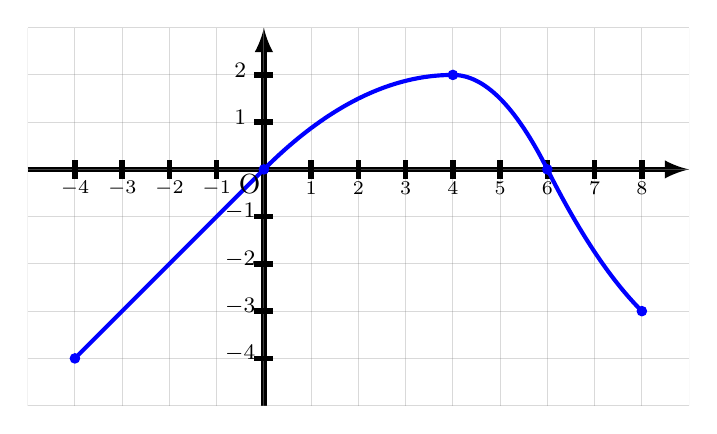
\begin{tikzpicture}[baseline,scale = 0.6]

    \tikzset{
      point/.style={
        thick,
        draw,
        cross out,
        inner sep=0pt,
        minimum width=5pt,
        minimum height=5pt,
      },
    }
    \clip (-5,-5) rectangle (9,3);
    	\draw[color ={black},line width = 2,>=latex,->] (-5,0)--(9,0);
	\draw[color ={black},line width = 2,>=latex,->] (0,-5)--(0,3);
	\draw[color ={gray},opacity = 0.3] (-5,0)--(9,0);
	\draw[color ={gray},opacity = 0.3] (-5,1)--(9,1);
	\draw[color ={gray},opacity = 0.3] (-5,2)--(9,2);
	\draw[color ={gray},opacity = 0.3] (-5,3)--(9,3);
	\draw[color ={gray},opacity = 0.3] (-5,0)--(9,0);
	\draw[color ={gray},opacity = 0.3] (-5,-1)--(9,-1);
	\draw[color ={gray},opacity = 0.3] (-5,-2)--(9,-2);
	\draw[color ={gray},opacity = 0.3] (-5,-3)--(9,-3);
	\draw[color ={gray},opacity = 0.3] (-5,-4)--(9,-4);
	\draw[color ={gray},opacity = 0.3] (-5,-5)--(9,-5);
	\draw[color ={gray},opacity = 0.3] (0,-5)--(0,3);
	\draw[color ={gray},opacity = 0.3] (1,-5)--(1,3);
	\draw[color ={gray},opacity = 0.3] (2,-5)--(2,3);
	\draw[color ={gray},opacity = 0.3] (3,-5)--(3,3);
	\draw[color ={gray},opacity = 0.3] (4,-5)--(4,3);
	\draw[color ={gray},opacity = 0.3] (5,-5)--(5,3);
	\draw[color ={gray},opacity = 0.3] (6,-5)--(6,3);
	\draw[color ={gray},opacity = 0.3] (7,-5)--(7,3);
	\draw[color ={gray},opacity = 0.3] (8,-5)--(8,3);
	\draw[color ={gray},opacity = 0.3] (9,-5)--(9,3);
	\draw[color ={gray},opacity = 0.3] (0,-5)--(0,3);
	\draw[color ={gray},opacity = 0.3] (-1,-5)--(-1,3);
	\draw[color ={gray},opacity = 0.3] (-2,-5)--(-2,3);
	\draw[color ={gray},opacity = 0.3] (-3,-5)--(-3,3);
	\draw[color ={gray},opacity = 0.3] (-4,-5)--(-4,3);
	\draw[color ={gray},opacity = 0.3] (-5,-5)--(-5,3);
	\draw[color ={black},line width = 2] (1,-0.2)--(1,0.2);
	\draw[color ={black},line width = 2] (2,-0.2)--(2,0.2);
	\draw[color ={black},line width = 2] (3,-0.2)--(3,0.2);
	\draw[color ={black},line width = 2] (4,-0.2)--(4,0.2);
	\draw[color ={black},line width = 2] (5,-0.2)--(5,0.2);
	\draw[color ={black},line width = 2] (6,-0.2)--(6,0.2);
	\draw[color ={black},line width = 2] (7,-0.2)--(7,0.2);
	\draw[color ={black},line width = 2] (8,-0.2)--(8,0.2);
	\draw[color ={black},line width = 2] (-1,-0.2)--(-1,0.2);
	\draw[color ={black},line width = 2] (-2,-0.2)--(-2,0.2);
	\draw[color ={black},line width = 2] (-3,-0.2)--(-3,0.2);
	\draw[color ={black},line width = 2] (-4,-0.2)--(-4,0.2);
	\draw[color ={black},line width = 2] (-0.2,1)--(0.2,1);
	\draw[color ={black},line width = 2] (-0.2,2)--(0.2,2);
	\draw[color ={black},line width = 2] (-0.2,-1)--(0.2,-1);
	\draw[color ={black},line width = 2] (-0.2,-2)--(0.2,-2);
	\draw[color ={black},line width = 2] (-0.2,-3)--(0.2,-3);
	\draw[color ={black},line width = 2] (-0.2,-4)--(0.2,-4);
	\draw (1,-0.4) node[anchor = center] {\scriptsize \color{black}{$1$}};
	\draw (2,-0.4) node[anchor = center] {\scriptsize \color{black}{$2$}};
	\draw (3,-0.4) node[anchor = center] {\scriptsize \color{black}{$3$}};
	\draw (4,-0.4) node[anchor = center] {\scriptsize \color{black}{$4$}};
	\draw (5,-0.4) node[anchor = center] {\scriptsize \color{black}{$5$}};
	\draw (6,-0.4) node[anchor = center] {\scriptsize \color{black}{$6$}};
	\draw (7,-0.4) node[anchor = center] {\scriptsize \color{black}{$7$}};
	\draw (8,-0.4) node[anchor = center] {\scriptsize \color{black}{$8$}};
	\draw (-1,-0.4) node[anchor = center] {\scriptsize \color{black}{$-1$}};
	\draw (-2,-0.4) node[anchor = center] {\scriptsize \color{black}{$-2$}};
	\draw (-3,-0.4) node[anchor = center] {\scriptsize \color{black}{$-3$}};
	\draw (-4,-0.4) node[anchor = center] {\scriptsize \color{black}{$-4$}};
	\draw (-0.5,1.1) node[anchor = center] {\footnotesize \color{black}{$1$}};
	\draw (-0.5,2.1) node[anchor = center] {\footnotesize \color{black}{$2$}};
	\draw (-0.5,-0.9) node[anchor = center] {\footnotesize \color{black}{$-1$}};
	\draw (-0.5,-1.9) node[anchor = center] {\footnotesize \color{black}{$-2$}};
	\draw (-0.5,-2.9) node[anchor = center] {\footnotesize \color{black}{$-3$}};
	\draw (-0.5,-3.9) node[anchor = center] {\footnotesize \color{black}{$-4$}};
	
	\draw[color = {blue},line width = 1.5, opacity = 1](-4,-4) .. controls +(1.33,1.33) and +(-1.33,-1.33)  .. (0.00,0.00)
 .. controls +(1.33,1.33) and +(-1.33,0.00)  .. (4.00,2.00)
 .. controls +(0.67,0.00) and +(-0.67,1.33)  .. (6.00,0.00)
 .. controls +(0.67,-1.33) and +(-0.67,0.67)  .. (8.00,-3.00)
;

	 \filldraw[color={blue},fill={{blue}}] (-4,-4) circle (0.1);
	 \filldraw[color={blue},fill={{blue}}] (0,0) circle (0.1);
	 \filldraw[color={blue},fill={{blue}}] (4,2) circle (0.1);
	 \filldraw[color={blue},fill={{blue}}] (6,0) circle (0.1);
	 \filldraw[color={blue},fill={{blue}}] (8,-3) circle (0.1);
	\draw [color={black}] (-0.3,-0.3) node[anchor = center,scale=1, rotate = 0] {O};

\end{tikzpicture} \end{minipage}
	\item \begin{minipage}[t]{\linewidth} Dresser le tableau de signes de la fonction $f$ représentée ci-dessous.\\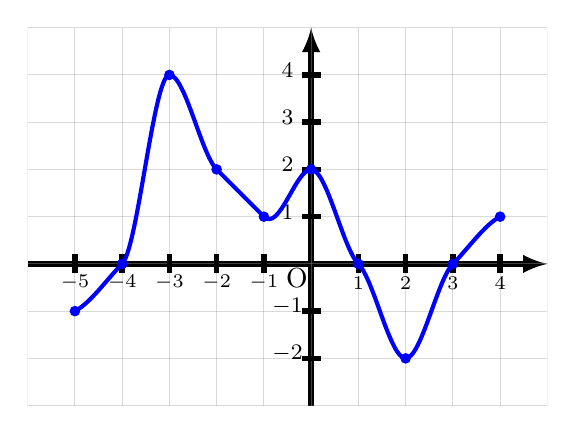
\begin{tikzpicture}[baseline,scale = 0.6]

    \tikzset{
      point/.style={
        thick,
        draw,
        cross out,
        inner sep=0pt,
        minimum width=5pt,
        minimum height=5pt,
      },
    }
    \clip (-6,-3) rectangle (5,5);
    	\draw[color ={black},line width = 2,>=latex,->] (-6,0)--(5,0);
	\draw[color ={black},line width = 2,>=latex,->] (0,-3)--(0,5);
	\draw[color ={gray},opacity = 0.3] (-6,0)--(5,0);
	\draw[color ={gray},opacity = 0.3] (-6,1)--(5,1);
	\draw[color ={gray},opacity = 0.3] (-6,2)--(5,2);
	\draw[color ={gray},opacity = 0.3] (-6,3)--(5,3);
	\draw[color ={gray},opacity = 0.3] (-6,4)--(5,4);
	\draw[color ={gray},opacity = 0.3] (-6,5)--(5,5);
	\draw[color ={gray},opacity = 0.3] (-6,0)--(5,0);
	\draw[color ={gray},opacity = 0.3] (-6,-1)--(5,-1);
	\draw[color ={gray},opacity = 0.3] (-6,-2)--(5,-2);
	\draw[color ={gray},opacity = 0.3] (-6,-3)--(5,-3);
	\draw[color ={gray},opacity = 0.3] (0,-3)--(0,5);
	\draw[color ={gray},opacity = 0.3] (1,-3)--(1,5);
	\draw[color ={gray},opacity = 0.3] (2,-3)--(2,5);
	\draw[color ={gray},opacity = 0.3] (3,-3)--(3,5);
	\draw[color ={gray},opacity = 0.3] (4,-3)--(4,5);
	\draw[color ={gray},opacity = 0.3] (5,-3)--(5,5);
	\draw[color ={gray},opacity = 0.3] (0,-3)--(0,5);
	\draw[color ={gray},opacity = 0.3] (-1,-3)--(-1,5);
	\draw[color ={gray},opacity = 0.3] (-2,-3)--(-2,5);
	\draw[color ={gray},opacity = 0.3] (-3,-3)--(-3,5);
	\draw[color ={gray},opacity = 0.3] (-4,-3)--(-4,5);
	\draw[color ={gray},opacity = 0.3] (-5,-3)--(-5,5);
	\draw[color ={gray},opacity = 0.3] (-6,-3)--(-6,5);
	\draw[color ={black},line width = 2] (1,-0.2)--(1,0.2);
	\draw[color ={black},line width = 2] (2,-0.2)--(2,0.2);
	\draw[color ={black},line width = 2] (3,-0.2)--(3,0.2);
	\draw[color ={black},line width = 2] (4,-0.2)--(4,0.2);
	\draw[color ={black},line width = 2] (-1,-0.2)--(-1,0.2);
	\draw[color ={black},line width = 2] (-2,-0.2)--(-2,0.2);
	\draw[color ={black},line width = 2] (-3,-0.2)--(-3,0.2);
	\draw[color ={black},line width = 2] (-4,-0.2)--(-4,0.2);
	\draw[color ={black},line width = 2] (-5,-0.2)--(-5,0.2);
	\draw[color ={black},line width = 2] (-0.2,1)--(0.2,1);
	\draw[color ={black},line width = 2] (-0.2,2)--(0.2,2);
	\draw[color ={black},line width = 2] (-0.2,3)--(0.2,3);
	\draw[color ={black},line width = 2] (-0.2,4)--(0.2,4);
	\draw[color ={black},line width = 2] (-0.2,-1)--(0.2,-1);
	\draw[color ={black},line width = 2] (-0.2,-2)--(0.2,-2);
	\draw (1,-0.4) node[anchor = center] {\scriptsize \color{black}{$1$}};
	\draw (2,-0.4) node[anchor = center] {\scriptsize \color{black}{$2$}};
	\draw (3,-0.4) node[anchor = center] {\scriptsize \color{black}{$3$}};
	\draw (4,-0.4) node[anchor = center] {\scriptsize \color{black}{$4$}};
	\draw (-1,-0.4) node[anchor = center] {\scriptsize \color{black}{$-1$}};
	\draw (-2,-0.4) node[anchor = center] {\scriptsize \color{black}{$-2$}};
	\draw (-3,-0.4) node[anchor = center] {\scriptsize \color{black}{$-3$}};
	\draw (-4,-0.4) node[anchor = center] {\scriptsize \color{black}{$-4$}};
	\draw (-5,-0.4) node[anchor = center] {\scriptsize \color{black}{$-5$}};
	\draw (-0.5,1.1) node[anchor = center] {\footnotesize \color{black}{$1$}};
	\draw (-0.5,2.1) node[anchor = center] {\footnotesize \color{black}{$2$}};
	\draw (-0.5,3.1) node[anchor = center] {\footnotesize \color{black}{$3$}};
	\draw (-0.5,4.1) node[anchor = center] {\footnotesize \color{black}{$4$}};
	\draw (-0.5,-0.9) node[anchor = center] {\footnotesize \color{black}{$-1$}};
	\draw (-0.5,-1.9) node[anchor = center] {\footnotesize \color{black}{$-2$}};
	
	\draw[color = {blue},line width = 1.5, opacity = 1](-5,-1) .. controls +(0.33,0.17) and +(-0.33,-0.33)  .. (-4.00,0.00)
 .. controls +(0.33,0.33) and +(-0.33,0.00)  .. (-3.00,4.00)
 .. controls +(0.33,0.00) and +(-0.33,0.33)  .. (-2.00,2.00)
 .. controls +(0.33,-0.33) and +(-0.33,0.33)  .. (-1.00,1.00)
 .. controls +(0.33,-0.33) and +(-0.33,0.00)  .. (0.00,2.00)
 .. controls +(0.33,0.00) and +(-0.33,0.33)  .. (1.00,0.00)
 .. controls +(0.33,-0.33) and +(-0.33,0.00)  .. (2.00,-2.00)
 .. controls +(0.33,0.00) and +(-0.33,-0.33)  .. (3.00,0.00)
 .. controls +(0.33,0.33) and +(-0.33,-0.17)  .. (4.00,1.00)
;

	 \filldraw[color={blue},fill={{blue}}] (-5,-1) circle (0.1);
	 \filldraw[color={blue},fill={{blue}}] (-4,0) circle (0.1);
	 \filldraw[color={blue},fill={{blue}}] (-3,4) circle (0.1);
	 \filldraw[color={blue},fill={{blue}}] (-2,2) circle (0.1);
	 \filldraw[color={blue},fill={{blue}}] (-1,1) circle (0.1);
	 \filldraw[color={blue},fill={{blue}}] (0,2) circle (0.1);
	 \filldraw[color={blue},fill={{blue}}] (1,0) circle (0.1);
	 \filldraw[color={blue},fill={{blue}}] (2,-2) circle (0.1);
	 \filldraw[color={blue},fill={{blue}}] (3,0) circle (0.1);
	 \filldraw[color={blue},fill={{blue}}] (4,1) circle (0.1);
	\draw [color={black}] (-0.3,-0.3) node[anchor = center,scale=1, rotate = 0] {O};

\end{tikzpicture} \end{minipage}
	\item \begin{minipage}[t]{\linewidth} Dresser le tableau de signes de la fonction $f$ représentée ci-dessous.\\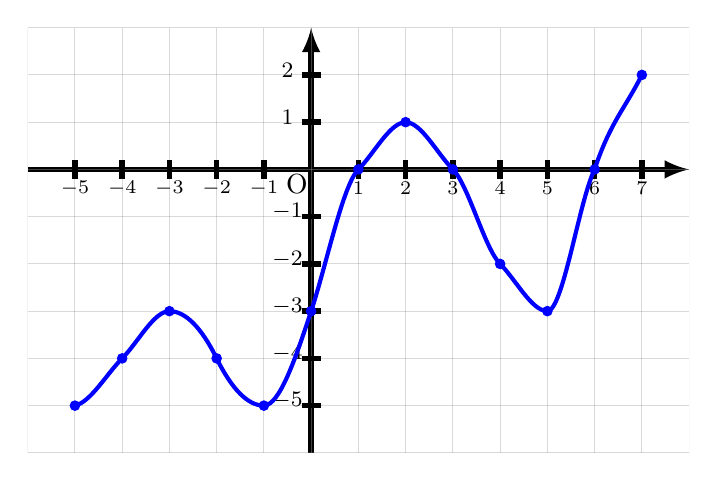
\begin{tikzpicture}[baseline,scale = 0.6]

    \tikzset{
      point/.style={
        thick,
        draw,
        cross out,
        inner sep=0pt,
        minimum width=5pt,
        minimum height=5pt,
      },
    }
    \clip (-6,-6) rectangle (8,3);
    	\draw[color ={black},line width = 2,>=latex,->] (-6,0)--(8,0);
	\draw[color ={black},line width = 2,>=latex,->] (0,-6)--(0,3);
	\draw[color ={gray},opacity = 0.3] (-6,0)--(8,0);
	\draw[color ={gray},opacity = 0.3] (-6,1)--(8,1);
	\draw[color ={gray},opacity = 0.3] (-6,2)--(8,2);
	\draw[color ={gray},opacity = 0.3] (-6,3)--(8,3);
	\draw[color ={gray},opacity = 0.3] (-6,0)--(8,0);
	\draw[color ={gray},opacity = 0.3] (-6,-1)--(8,-1);
	\draw[color ={gray},opacity = 0.3] (-6,-2)--(8,-2);
	\draw[color ={gray},opacity = 0.3] (-6,-3)--(8,-3);
	\draw[color ={gray},opacity = 0.3] (-6,-4)--(8,-4);
	\draw[color ={gray},opacity = 0.3] (-6,-5)--(8,-5);
	\draw[color ={gray},opacity = 0.3] (-6,-6)--(8,-6);
	\draw[color ={gray},opacity = 0.3] (0,-6)--(0,3);
	\draw[color ={gray},opacity = 0.3] (1,-6)--(1,3);
	\draw[color ={gray},opacity = 0.3] (2,-6)--(2,3);
	\draw[color ={gray},opacity = 0.3] (3,-6)--(3,3);
	\draw[color ={gray},opacity = 0.3] (4,-6)--(4,3);
	\draw[color ={gray},opacity = 0.3] (5,-6)--(5,3);
	\draw[color ={gray},opacity = 0.3] (6,-6)--(6,3);
	\draw[color ={gray},opacity = 0.3] (7,-6)--(7,3);
	\draw[color ={gray},opacity = 0.3] (8,-6)--(8,3);
	\draw[color ={gray},opacity = 0.3] (0,-6)--(0,3);
	\draw[color ={gray},opacity = 0.3] (-1,-6)--(-1,3);
	\draw[color ={gray},opacity = 0.3] (-2,-6)--(-2,3);
	\draw[color ={gray},opacity = 0.3] (-3,-6)--(-3,3);
	\draw[color ={gray},opacity = 0.3] (-4,-6)--(-4,3);
	\draw[color ={gray},opacity = 0.3] (-5,-6)--(-5,3);
	\draw[color ={gray},opacity = 0.3] (-6,-6)--(-6,3);
	\draw[color ={black},line width = 2] (1,-0.2)--(1,0.2);
	\draw[color ={black},line width = 2] (2,-0.2)--(2,0.2);
	\draw[color ={black},line width = 2] (3,-0.2)--(3,0.2);
	\draw[color ={black},line width = 2] (4,-0.2)--(4,0.2);
	\draw[color ={black},line width = 2] (5,-0.2)--(5,0.2);
	\draw[color ={black},line width = 2] (6,-0.2)--(6,0.2);
	\draw[color ={black},line width = 2] (7,-0.2)--(7,0.2);
	\draw[color ={black},line width = 2] (-1,-0.2)--(-1,0.2);
	\draw[color ={black},line width = 2] (-2,-0.2)--(-2,0.2);
	\draw[color ={black},line width = 2] (-3,-0.2)--(-3,0.2);
	\draw[color ={black},line width = 2] (-4,-0.2)--(-4,0.2);
	\draw[color ={black},line width = 2] (-5,-0.2)--(-5,0.2);
	\draw[color ={black},line width = 2] (-0.2,1)--(0.2,1);
	\draw[color ={black},line width = 2] (-0.2,2)--(0.2,2);
	\draw[color ={black},line width = 2] (-0.2,-1)--(0.2,-1);
	\draw[color ={black},line width = 2] (-0.2,-2)--(0.2,-2);
	\draw[color ={black},line width = 2] (-0.2,-3)--(0.2,-3);
	\draw[color ={black},line width = 2] (-0.2,-4)--(0.2,-4);
	\draw[color ={black},line width = 2] (-0.2,-5)--(0.2,-5);
	\draw (1,-0.4) node[anchor = center] {\scriptsize \color{black}{$1$}};
	\draw (2,-0.4) node[anchor = center] {\scriptsize \color{black}{$2$}};
	\draw (3,-0.4) node[anchor = center] {\scriptsize \color{black}{$3$}};
	\draw (4,-0.4) node[anchor = center] {\scriptsize \color{black}{$4$}};
	\draw (5,-0.4) node[anchor = center] {\scriptsize \color{black}{$5$}};
	\draw (6,-0.4) node[anchor = center] {\scriptsize \color{black}{$6$}};
	\draw (7,-0.4) node[anchor = center] {\scriptsize \color{black}{$7$}};
	\draw (-1,-0.4) node[anchor = center] {\scriptsize \color{black}{$-1$}};
	\draw (-2,-0.4) node[anchor = center] {\scriptsize \color{black}{$-2$}};
	\draw (-3,-0.4) node[anchor = center] {\scriptsize \color{black}{$-3$}};
	\draw (-4,-0.4) node[anchor = center] {\scriptsize \color{black}{$-4$}};
	\draw (-5,-0.4) node[anchor = center] {\scriptsize \color{black}{$-5$}};
	\draw (-0.5,1.1) node[anchor = center] {\footnotesize \color{black}{$1$}};
	\draw (-0.5,2.1) node[anchor = center] {\footnotesize \color{black}{$2$}};
	\draw (-0.5,-0.9) node[anchor = center] {\footnotesize \color{black}{$-1$}};
	\draw (-0.5,-1.9) node[anchor = center] {\footnotesize \color{black}{$-2$}};
	\draw (-0.5,-2.9) node[anchor = center] {\footnotesize \color{black}{$-3$}};
	\draw (-0.5,-3.9) node[anchor = center] {\footnotesize \color{black}{$-4$}};
	\draw (-0.5,-4.9) node[anchor = center] {\footnotesize \color{black}{$-5$}};
	
	\draw[color = {blue},line width = 1.5, opacity = 1](-5,-5) .. controls +(0.33,0.07) and +(-0.33,-0.33)  .. (-4.00,-4.00)
 .. controls +(0.33,0.33) and +(-0.33,0.00)  .. (-3.00,-3.00)
 .. controls +(0.33,0.00) and +(-0.33,0.67)  .. (-2.00,-4.00)
 .. controls +(0.33,-0.67) and +(-0.33,0.00)  .. (-1.00,-5.00)
 .. controls +(0.33,0.00) and +(-0.33,-1.00)  .. (0.00,-3.00)
 .. controls +(0.33,1.00) and +(-0.33,-0.33)  .. (1.00,0.00)
 .. controls +(0.33,0.33) and +(-0.33,0.00)  .. (2.00,1.00)
 .. controls +(0.33,0.00) and +(-0.33,0.33)  .. (3.00,0.00)
 .. controls +(0.33,-0.33) and +(-0.33,0.33)  .. (4.00,-2.00)
 .. controls +(0.33,-0.33) and +(-0.33,0.00)  .. (5.00,-3.00)
 .. controls +(0.33,0.00) and +(-0.33,-0.67)  .. (6.00,0.00)
 .. controls +(0.33,1.00) and +(-0.33,-0.67)  .. (7.00,2.00)
;

	 \filldraw[color={blue},fill={{blue}}] (-5,-5) circle (0.1);
	 \filldraw[color={blue},fill={{blue}}] (-4,-4) circle (0.1);
	 \filldraw[color={blue},fill={{blue}}] (-3,-3) circle (0.1);
	 \filldraw[color={blue},fill={{blue}}] (-2,-4) circle (0.1);
	 \filldraw[color={blue},fill={{blue}}] (-1,-5) circle (0.1);
	 \filldraw[color={blue},fill={{blue}}] (0,-3) circle (0.1);
	 \filldraw[color={blue},fill={{blue}}] (1,0) circle (0.1);
	 \filldraw[color={blue},fill={{blue}}] (2,1) circle (0.1);
	 \filldraw[color={blue},fill={{blue}}] (3,0) circle (0.1);
	 \filldraw[color={blue},fill={{blue}}] (4,-2) circle (0.1);
	 \filldraw[color={blue},fill={{blue}}] (5,-3) circle (0.1);
	 \filldraw[color={blue},fill={{blue}}] (6,0) circle (0.1);
	 \filldraw[color={blue},fill={{blue}}] (7,2) circle (0.1);
	\draw [color={black}] (-0.3,-0.3) node[anchor = center,scale=1, rotate = 0] {O};

\end{tikzpicture} \end{minipage}
	\item \begin{minipage}[t]{\linewidth} Dresser le tableau de signes de la fonction $f$ représentée ci-dessous.\\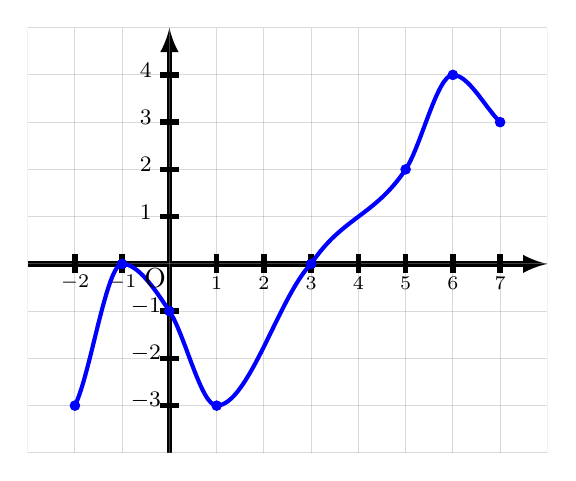
\begin{tikzpicture}[baseline,scale = 0.6]

    \tikzset{
      point/.style={
        thick,
        draw,
        cross out,
        inner sep=0pt,
        minimum width=5pt,
        minimum height=5pt,
      },
    }
    \clip (-3,-4) rectangle (8,5);
    	\draw[color ={black},line width = 2,>=latex,->] (-3,0)--(8,0);
	\draw[color ={black},line width = 2,>=latex,->] (0,-4)--(0,5);
	\draw[color ={gray},opacity = 0.3] (-3,0)--(8,0);
	\draw[color ={gray},opacity = 0.3] (-3,1)--(8,1);
	\draw[color ={gray},opacity = 0.3] (-3,2)--(8,2);
	\draw[color ={gray},opacity = 0.3] (-3,3)--(8,3);
	\draw[color ={gray},opacity = 0.3] (-3,4)--(8,4);
	\draw[color ={gray},opacity = 0.3] (-3,5)--(8,5);
	\draw[color ={gray},opacity = 0.3] (-3,0)--(8,0);
	\draw[color ={gray},opacity = 0.3] (-3,-1)--(8,-1);
	\draw[color ={gray},opacity = 0.3] (-3,-2)--(8,-2);
	\draw[color ={gray},opacity = 0.3] (-3,-3)--(8,-3);
	\draw[color ={gray},opacity = 0.3] (-3,-4)--(8,-4);
	\draw[color ={gray},opacity = 0.3] (0,-4)--(0,5);
	\draw[color ={gray},opacity = 0.3] (1,-4)--(1,5);
	\draw[color ={gray},opacity = 0.3] (2,-4)--(2,5);
	\draw[color ={gray},opacity = 0.3] (3,-4)--(3,5);
	\draw[color ={gray},opacity = 0.3] (4,-4)--(4,5);
	\draw[color ={gray},opacity = 0.3] (5,-4)--(5,5);
	\draw[color ={gray},opacity = 0.3] (6,-4)--(6,5);
	\draw[color ={gray},opacity = 0.3] (7,-4)--(7,5);
	\draw[color ={gray},opacity = 0.3] (8,-4)--(8,5);
	\draw[color ={gray},opacity = 0.3] (0,-4)--(0,5);
	\draw[color ={gray},opacity = 0.3] (-1,-4)--(-1,5);
	\draw[color ={gray},opacity = 0.3] (-2,-4)--(-2,5);
	\draw[color ={gray},opacity = 0.3] (-3,-4)--(-3,5);
	\draw[color ={black},line width = 2] (1,-0.2)--(1,0.2);
	\draw[color ={black},line width = 2] (2,-0.2)--(2,0.2);
	\draw[color ={black},line width = 2] (3,-0.2)--(3,0.2);
	\draw[color ={black},line width = 2] (4,-0.2)--(4,0.2);
	\draw[color ={black},line width = 2] (5,-0.2)--(5,0.2);
	\draw[color ={black},line width = 2] (6,-0.2)--(6,0.2);
	\draw[color ={black},line width = 2] (7,-0.2)--(7,0.2);
	\draw[color ={black},line width = 2] (-1,-0.2)--(-1,0.2);
	\draw[color ={black},line width = 2] (-2,-0.2)--(-2,0.2);
	\draw[color ={black},line width = 2] (-0.2,1)--(0.2,1);
	\draw[color ={black},line width = 2] (-0.2,2)--(0.2,2);
	\draw[color ={black},line width = 2] (-0.2,3)--(0.2,3);
	\draw[color ={black},line width = 2] (-0.2,4)--(0.2,4);
	\draw[color ={black},line width = 2] (-0.2,-1)--(0.2,-1);
	\draw[color ={black},line width = 2] (-0.2,-2)--(0.2,-2);
	\draw[color ={black},line width = 2] (-0.2,-3)--(0.2,-3);
	\draw (1,-0.4) node[anchor = center] {\scriptsize \color{black}{$1$}};
	\draw (2,-0.4) node[anchor = center] {\scriptsize \color{black}{$2$}};
	\draw (3,-0.4) node[anchor = center] {\scriptsize \color{black}{$3$}};
	\draw (4,-0.4) node[anchor = center] {\scriptsize \color{black}{$4$}};
	\draw (5,-0.4) node[anchor = center] {\scriptsize \color{black}{$5$}};
	\draw (6,-0.4) node[anchor = center] {\scriptsize \color{black}{$6$}};
	\draw (7,-0.4) node[anchor = center] {\scriptsize \color{black}{$7$}};
	\draw (-1,-0.4) node[anchor = center] {\scriptsize \color{black}{$-1$}};
	\draw (-2,-0.4) node[anchor = center] {\scriptsize \color{black}{$-2$}};
	\draw (-0.5,1.1) node[anchor = center] {\footnotesize \color{black}{$1$}};
	\draw (-0.5,2.1) node[anchor = center] {\footnotesize \color{black}{$2$}};
	\draw (-0.5,3.1) node[anchor = center] {\footnotesize \color{black}{$3$}};
	\draw (-0.5,4.1) node[anchor = center] {\footnotesize \color{black}{$4$}};
	\draw (-0.5,-0.9) node[anchor = center] {\footnotesize \color{black}{$-1$}};
	\draw (-0.5,-1.9) node[anchor = center] {\footnotesize \color{black}{$-2$}};
	\draw (-0.5,-2.9) node[anchor = center] {\footnotesize \color{black}{$-3$}};
	
	\draw[color = {blue},line width = 1.5, opacity = 1](-2,-3) .. controls +(0.33,0.67) and +(-0.33,0.00)  .. (-1.00,0.00)
 .. controls +(0.33,0.00) and +(-0.33,0.50)  .. (0.00,-1.00)
 .. controls +(0.33,-0.50) and +(-0.33,0.00)  .. (1.00,-3.00)
 .. controls +(0.67,0.00) and +(-0.67,-0.67)  .. (3.00,0.00)
 .. controls +(0.67,1.00) and +(-0.67,-1.00)  .. (5.00,2.00)
 .. controls +(0.33,0.50) and +(-0.33,0.00)  .. (6.00,4.00)
 .. controls +(0.33,0.00) and +(-0.33,0.33)  .. (7.00,3.00)
;

	 \filldraw[color={blue},fill={{blue}}] (-2,-3) circle (0.1);
	 \filldraw[color={blue},fill={{blue}}] (-1,0) circle (0.1);
	 \filldraw[color={blue},fill={{blue}}] (0,-1) circle (0.1);
	 \filldraw[color={blue},fill={{blue}}] (1,-3) circle (0.1);
	 \filldraw[color={blue},fill={{blue}}] (3,0) circle (0.1);
	 \filldraw[color={blue},fill={{blue}}] (5,2) circle (0.1);
	 \filldraw[color={blue},fill={{blue}}] (6,4) circle (0.1);
	 \filldraw[color={blue},fill={{blue}}] (7,3) circle (0.1);
	\draw [color={black}] (-0.3,-0.3) node[anchor = center,scale=1, rotate = 0] {O};

\end{tikzpicture} \end{minipage}
\end{enumerate}
\end{multicols}
\end{exercice}

\end{document}
